\subsection{Tabular data}

Instead of monitoring the median result, we can also look for the best one in each sweep, along with the average runtime. The results are also report graphically in Fig.~\ref{fig:apptabular}. The hyper-parameters are reported in Table~\ref{tab:tabularhyperparams}.      

\begin{table*}
    \centering
    \small
    \begin{tabular}{|p{1cm}>{\raggedleft\arraybackslash}p{1cm}>{\raggedleft\arraybackslash}p{0.8cm}p{0.6cm}|cc|cc|}
        \hline
         \multirow{2}{*}{Dataset} & \multirow{2}{*}{Samples} & \multirow{2}{*}{Features} & \multirow{2}{*}{$\delta$} & \multicolumn{2}{c|}{Validation AUROC $\uparrow$} & \multicolumn{2}{c|}{Wallclock Runtime (s) $\downarrow$}\\
                 &            &             &          & \makecell{DP-SGD} & \makecell{Clipless\\ DP-SGD} &  \makecell{DP-SGD} & \makecell{Clipless\\ DP-SGD}\\
        \hline
        \hline
ALOI & 39,627 & 27 & $10^{-5}$ & $\textbf{56.5}$ & $56.2$ & $159.1$ & $\textbf{11.3}$\\
campaign & 32,950 & 62 & $10^{-5}$ & $\textbf{90.0}$ & $82.2$ & $155.6$ & $\textbf{11.8}$\\
celeba & 162,079 & 39 & $10^{-6}$ & $\textbf{96.6}$ & $96.5$ & $41.1$ & $\textbf{34.6}$\\
census & 239,428 & 500 & $10^{-6}$ & $\textbf{93.3}$ & $92.5$ & $820.0$ & $\textbf{79.8}$\\
donors & 495,460 & 10 & $10^{-6}$ & $100.0$ & $\textbf{100.0}$ & $257.9$ & $\textbf{90.2}$\\
magic & 15,216 & 10 & $10^{-5}$ & $\textbf{90.7}$ & $89.7$ & $89.9$ & $\textbf{56.0}$\\
shuttle & 39,277 & 9 & $10^{-5}$ & $98.3$ & $\textbf{99.4}$ & $11.1$ & $\textbf{6.8}$\\
skin & 196,045 & 3 & $10^{-6}$ & $\textbf{100.0}$ & $99.8$ & $54.2$ & $\textbf{40.2}$\\
yeast & 1,187 & 8 & $10^{-4}$ & $66.8$ & $\textbf{75.1}$ & $22.1$ & $\textbf{5.6}$\\
        \hline
    \end{tabular}
    \caption{Best validation AUROC values (in \%) for models trained under \DP privacy with $\epsilon=1$, with DP-SGD and Clipless DP-SGD, on binary classification tasks of tabular data from Adbench datasets~\cite{han2022adbench}. We use a random 80/20\% stratified split into train/val.}
    \label{app:tabularutilityruntime}
\end{table*}

\begin{figure}
    \centering
    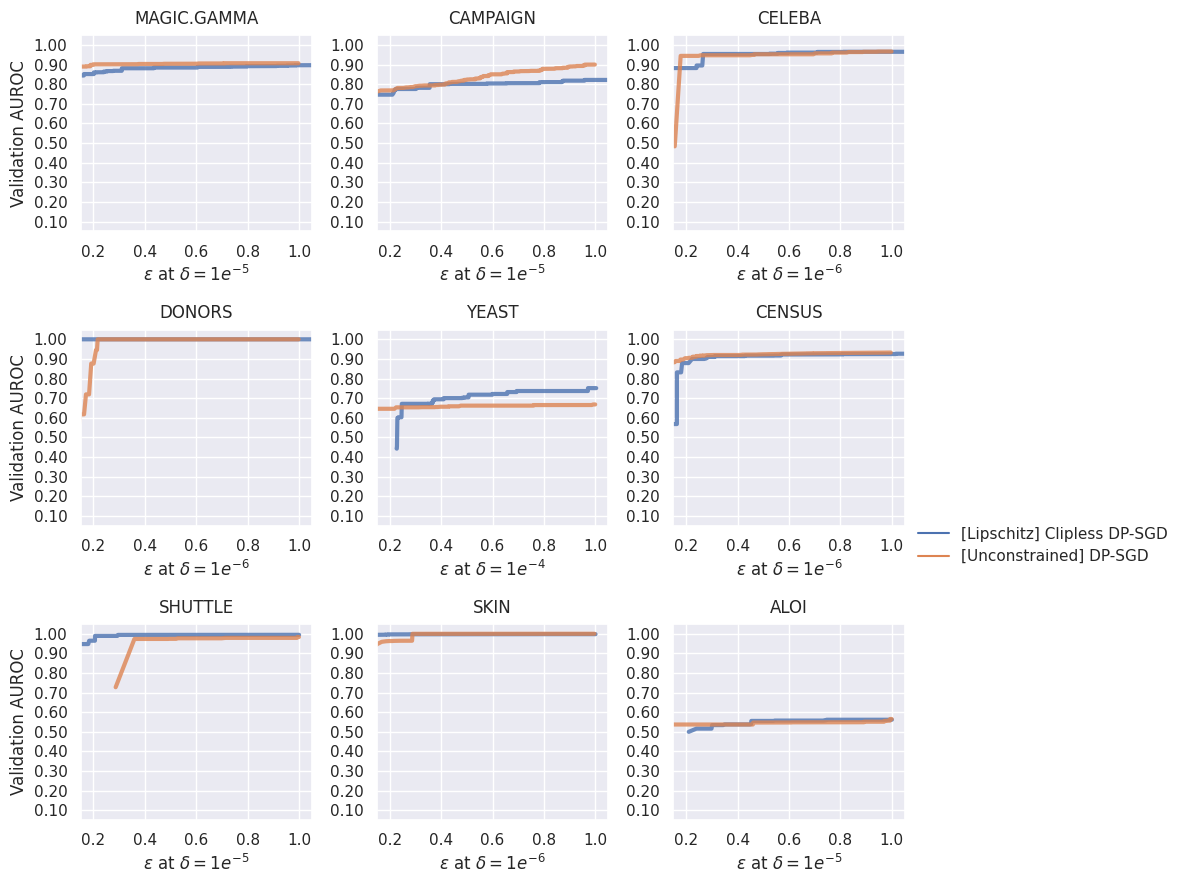
\includegraphics[width=1\linewidth]{figures/tabular.png}
    \caption{\textbf{Pareto front of AUROC values} on tabular data.}
    \label{fig:apptabular}
\end{figure}

\begin{table}
\centering
\begin{tabular}{|c c c|} 
 \hline
 Hyper-Parameter & Minimum Value & Maximum Value \\ [0.5ex] 
 \hline\hline
 Input Clipping & \multicolumn{2}{c|}{None} \\ 
 \hline
 Batch Size & $512$ & $10^4$ \\
 \hline
 Loss Gradient Clipping & \multicolumn{2}{c|}{automatic (90\%-th percentile)} \\
 \hline
 $\tau$ (BCE) & $10^{-2}$ & $100$\\
 \hline
 Learning Rate & 0.00001 & 1.0\\
 \hline
\end{tabular}
\caption{\textbf{Hyper-parameters of Clipless DP-SGD for the Tabular experiment.}}
\label{tab:tabularhyperparams}
\end{table}

\subsection{Pareto fronts}

\begin{figure}
\begin{subfigure}{.33\columnwidth}
        \centering
        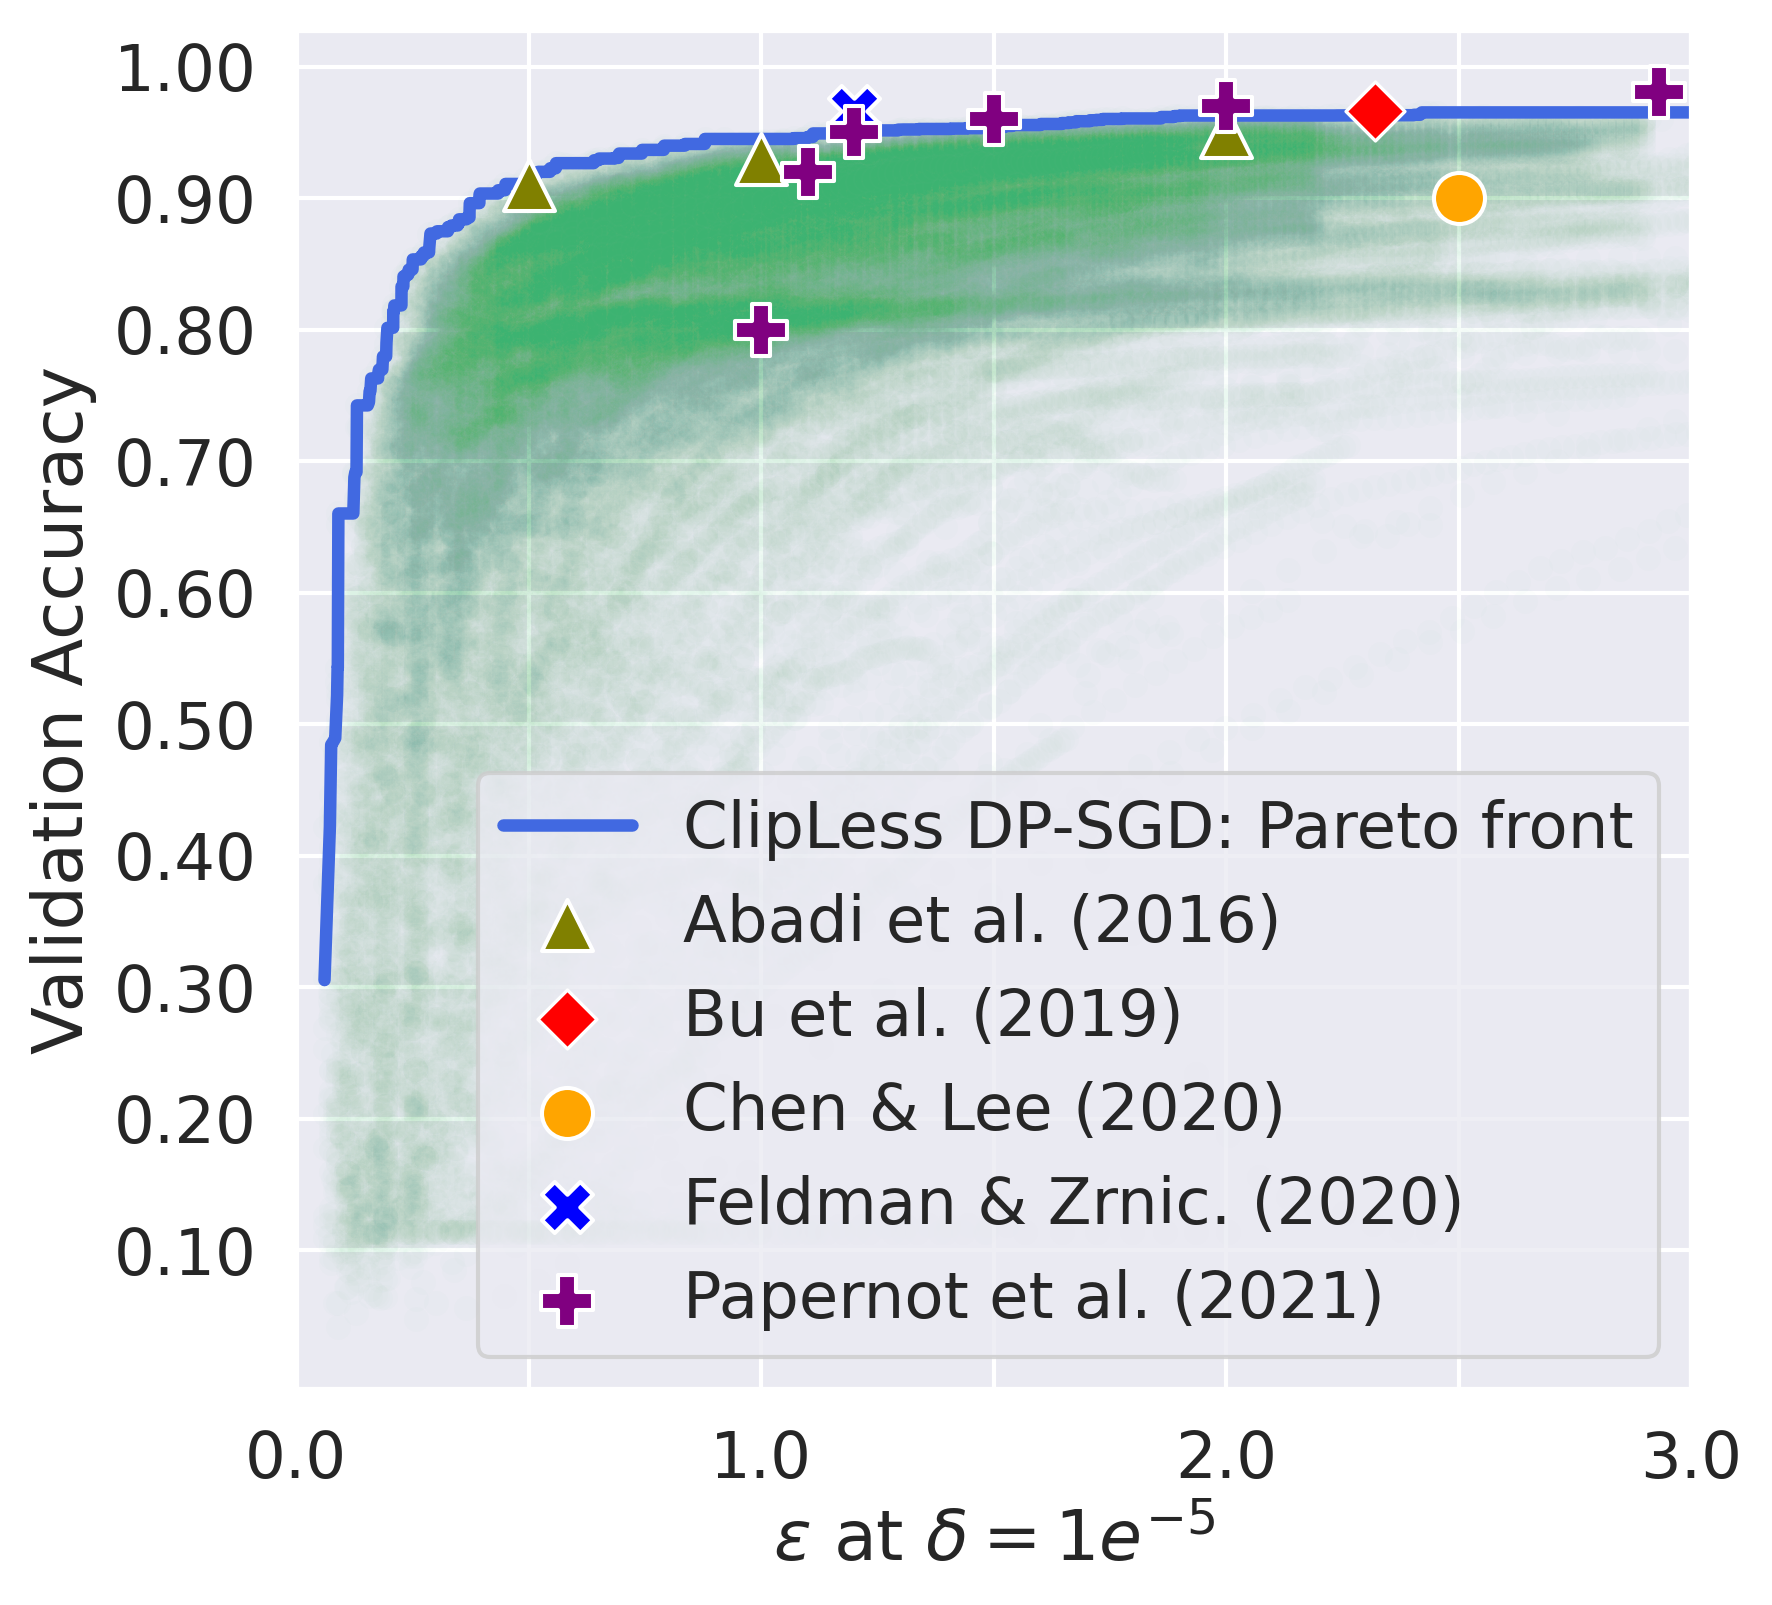
\includegraphics[width=\linewidth]{figures/mnist.png}
        \caption{\textbf{MNIST}.}
        \label{fig:paretofrontmnist}
    \end{subfigure}
    %\hfil
    \begin{subfigure}{.33\columnwidth}
        \centering
        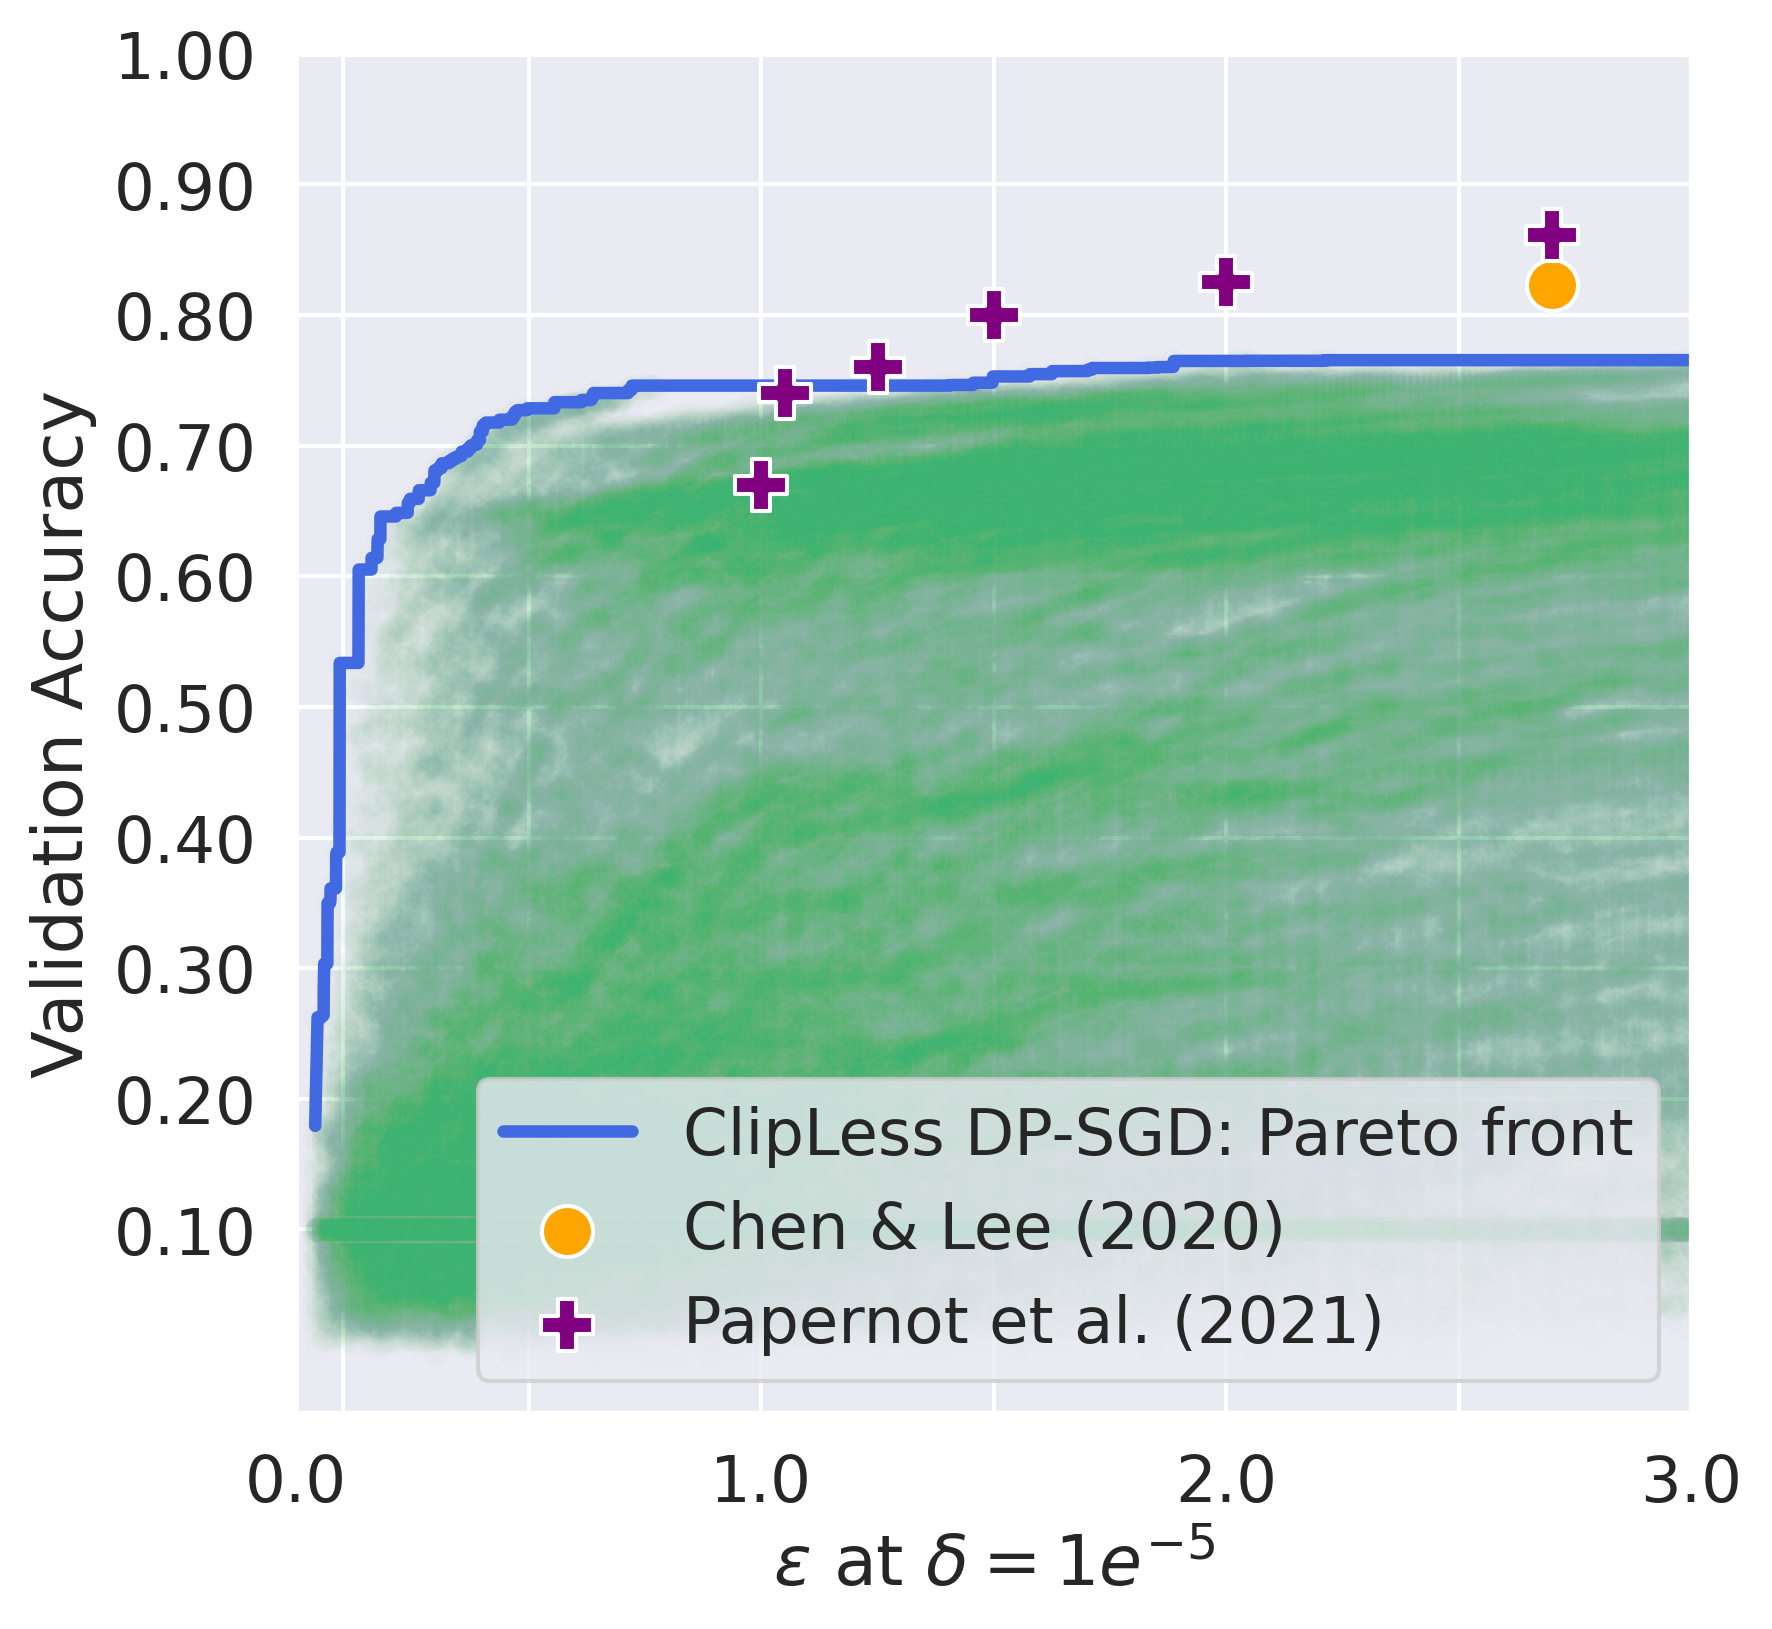
\includegraphics[width=\linewidth]{figures/fashion.png}
        \caption{\textbf{F-MNIST}.}
        \label{fig:paretofrontfashion}
    \end{subfigure}
    %\hfil
    \begin{subfigure}{.33\columnwidth}
        \centering
        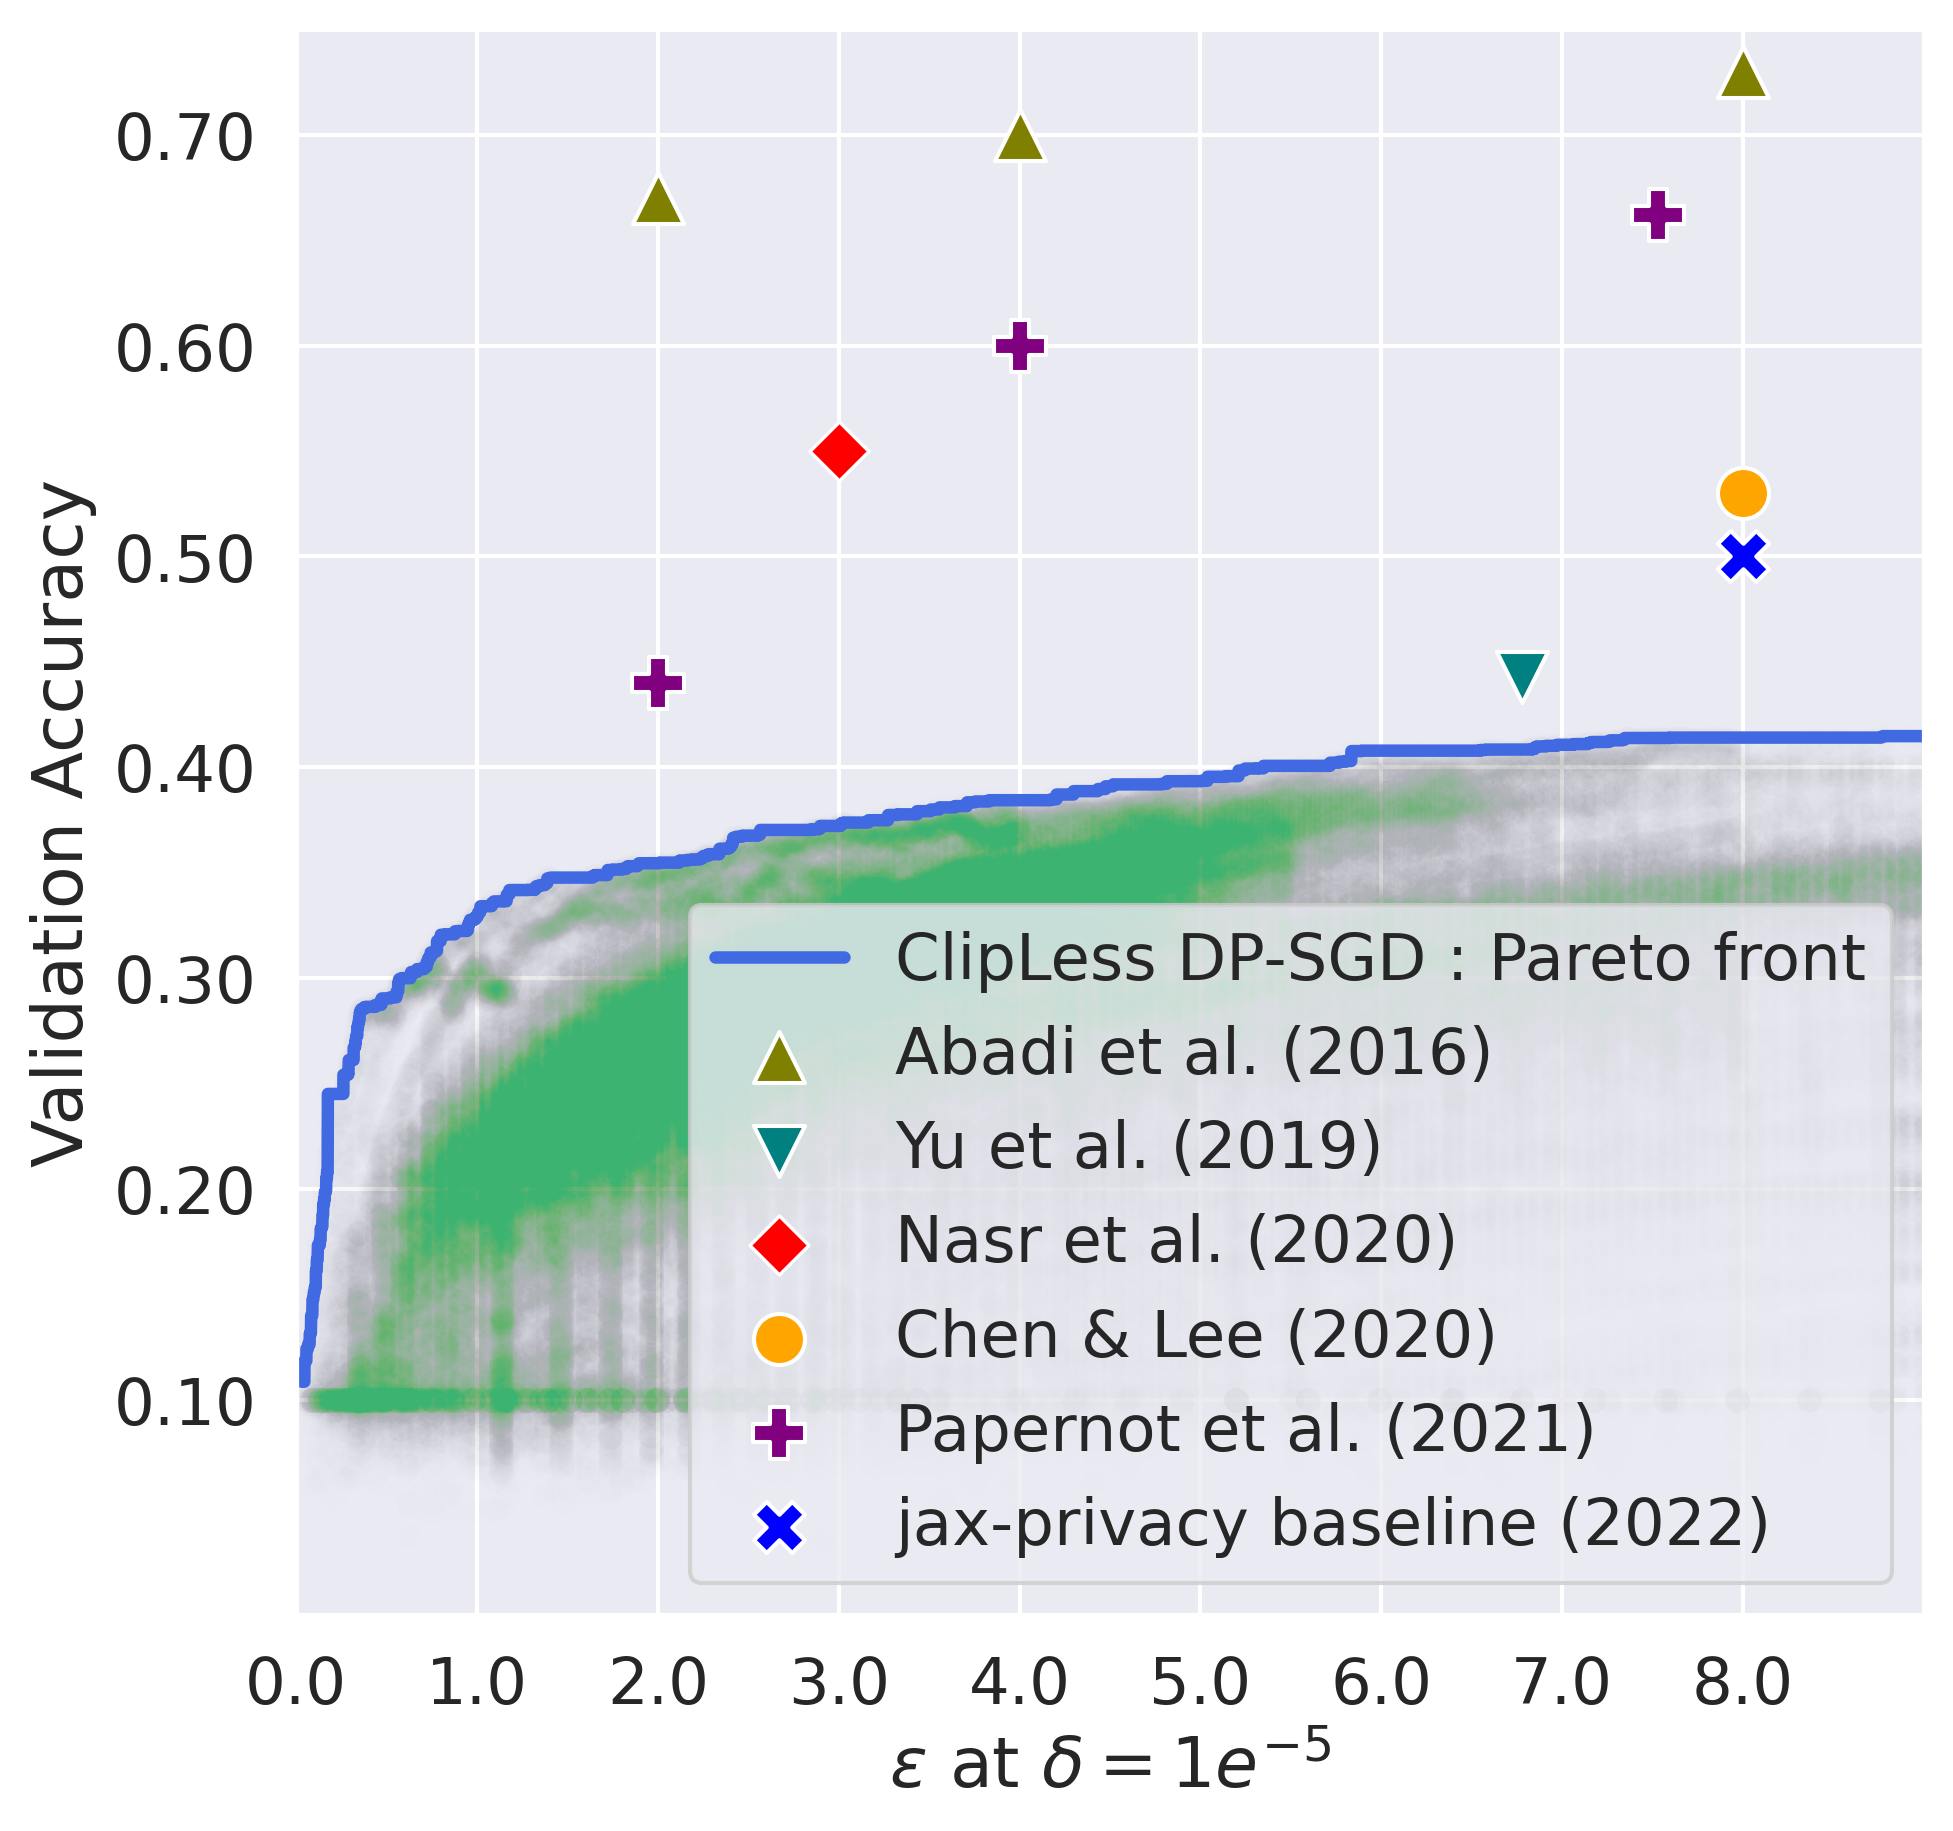
\includegraphics[width=\linewidth]{figures/cifar10.png}
        \caption{\textbf{CIFAR-10}.}
        \label{fig:paretofrontcifar}
    \end{subfigure}
    \caption{\textbf{Our framework paints a clearer picture of the privacy/utility trade-off.} We trained models in an "out of the box setting" (no pre-training, no data augmentation and no handcrafted features) on multiple tasks. Each green dot corresponds to an (\textbf{accuracy}, $\epsilon$) pair from an epoch of one of the runs, while the blue line is the Pareto front (convex hull of all the dots).  
    While our results align with the baselines presented in other frameworks, we recognize the importance of domain-specific engineering. In this regard, we find the innovations introduced in ~\cite{papernot2021tempered,tramer2021differentially,de2022unlocking} and references therein highly relevant. These advancements demonstrate compatibility with our framework and hold potential for future integration.
    %We reported the validation accuracy with respect to the \mbox{$(\epsilon,10^{-5})-\text{DP}$} guarantees provided.
    %While our results are comparable to the baselines presented in other frameworks, we emphasize the significance of domain specific engineering by showcasing results from~\cite{papernot2021tempered,tramèr2021differentially,de2022unlocking} and references therein. Some of these %Results of vanilla DP-SGD are reported in fig \ref{app:dropinreplacement}~\ref{fig:vaniallgnp}
    }\label{fig:paretofront}
\end{figure}

We rely on Bayesian optimization~\cite{snoek2012practical} with Hyper-band~\cite{li2017hyperband} heuristic for early stopping. The influence of some hyperparameters has to be highlighted to facilitate training with our framework, therefore we provide a table that provides insights into the effects of principal hyperparameters in Figure~\ref{fig:hyperparams}. Most hyper-parameters extend over different scales (such as the learning rate), so they are sampled according to log-uniform distribution, to ensure fair covering of the search space. Additionnaly, the importance of the softmax cross-entropy temperature $\tau$ has been demonstrated in previous work~\cite{bethune2022pay}.

\begin{figure}
    \centering
        \begin{tabular}{|p{3.5cm}|p{5.5cm}p{5cm}|}
        \hline
        \textbf{Hyperparameter \newline Tuning} & \textbf{Influence on utility} & \textbf{Influence on privacy \newline leakage per step} \\
        \hline
        \hline
        Increasing Batch Size & Beneficial: decreases the sensitivity. & Detrimental: reduces the privacy amplification by subsampling. \\
        \hline
        Loss Gradient Clipping & Beneficial: tighter sensitivity bounds. \newline Detrimental: biases the direction of the gradient. & No influence \\
        \hline
        Clipping Input Norms & Detrimental: destroy information, but may increases generalization & No influence \\
        \hline
        \end{tabular}


    % 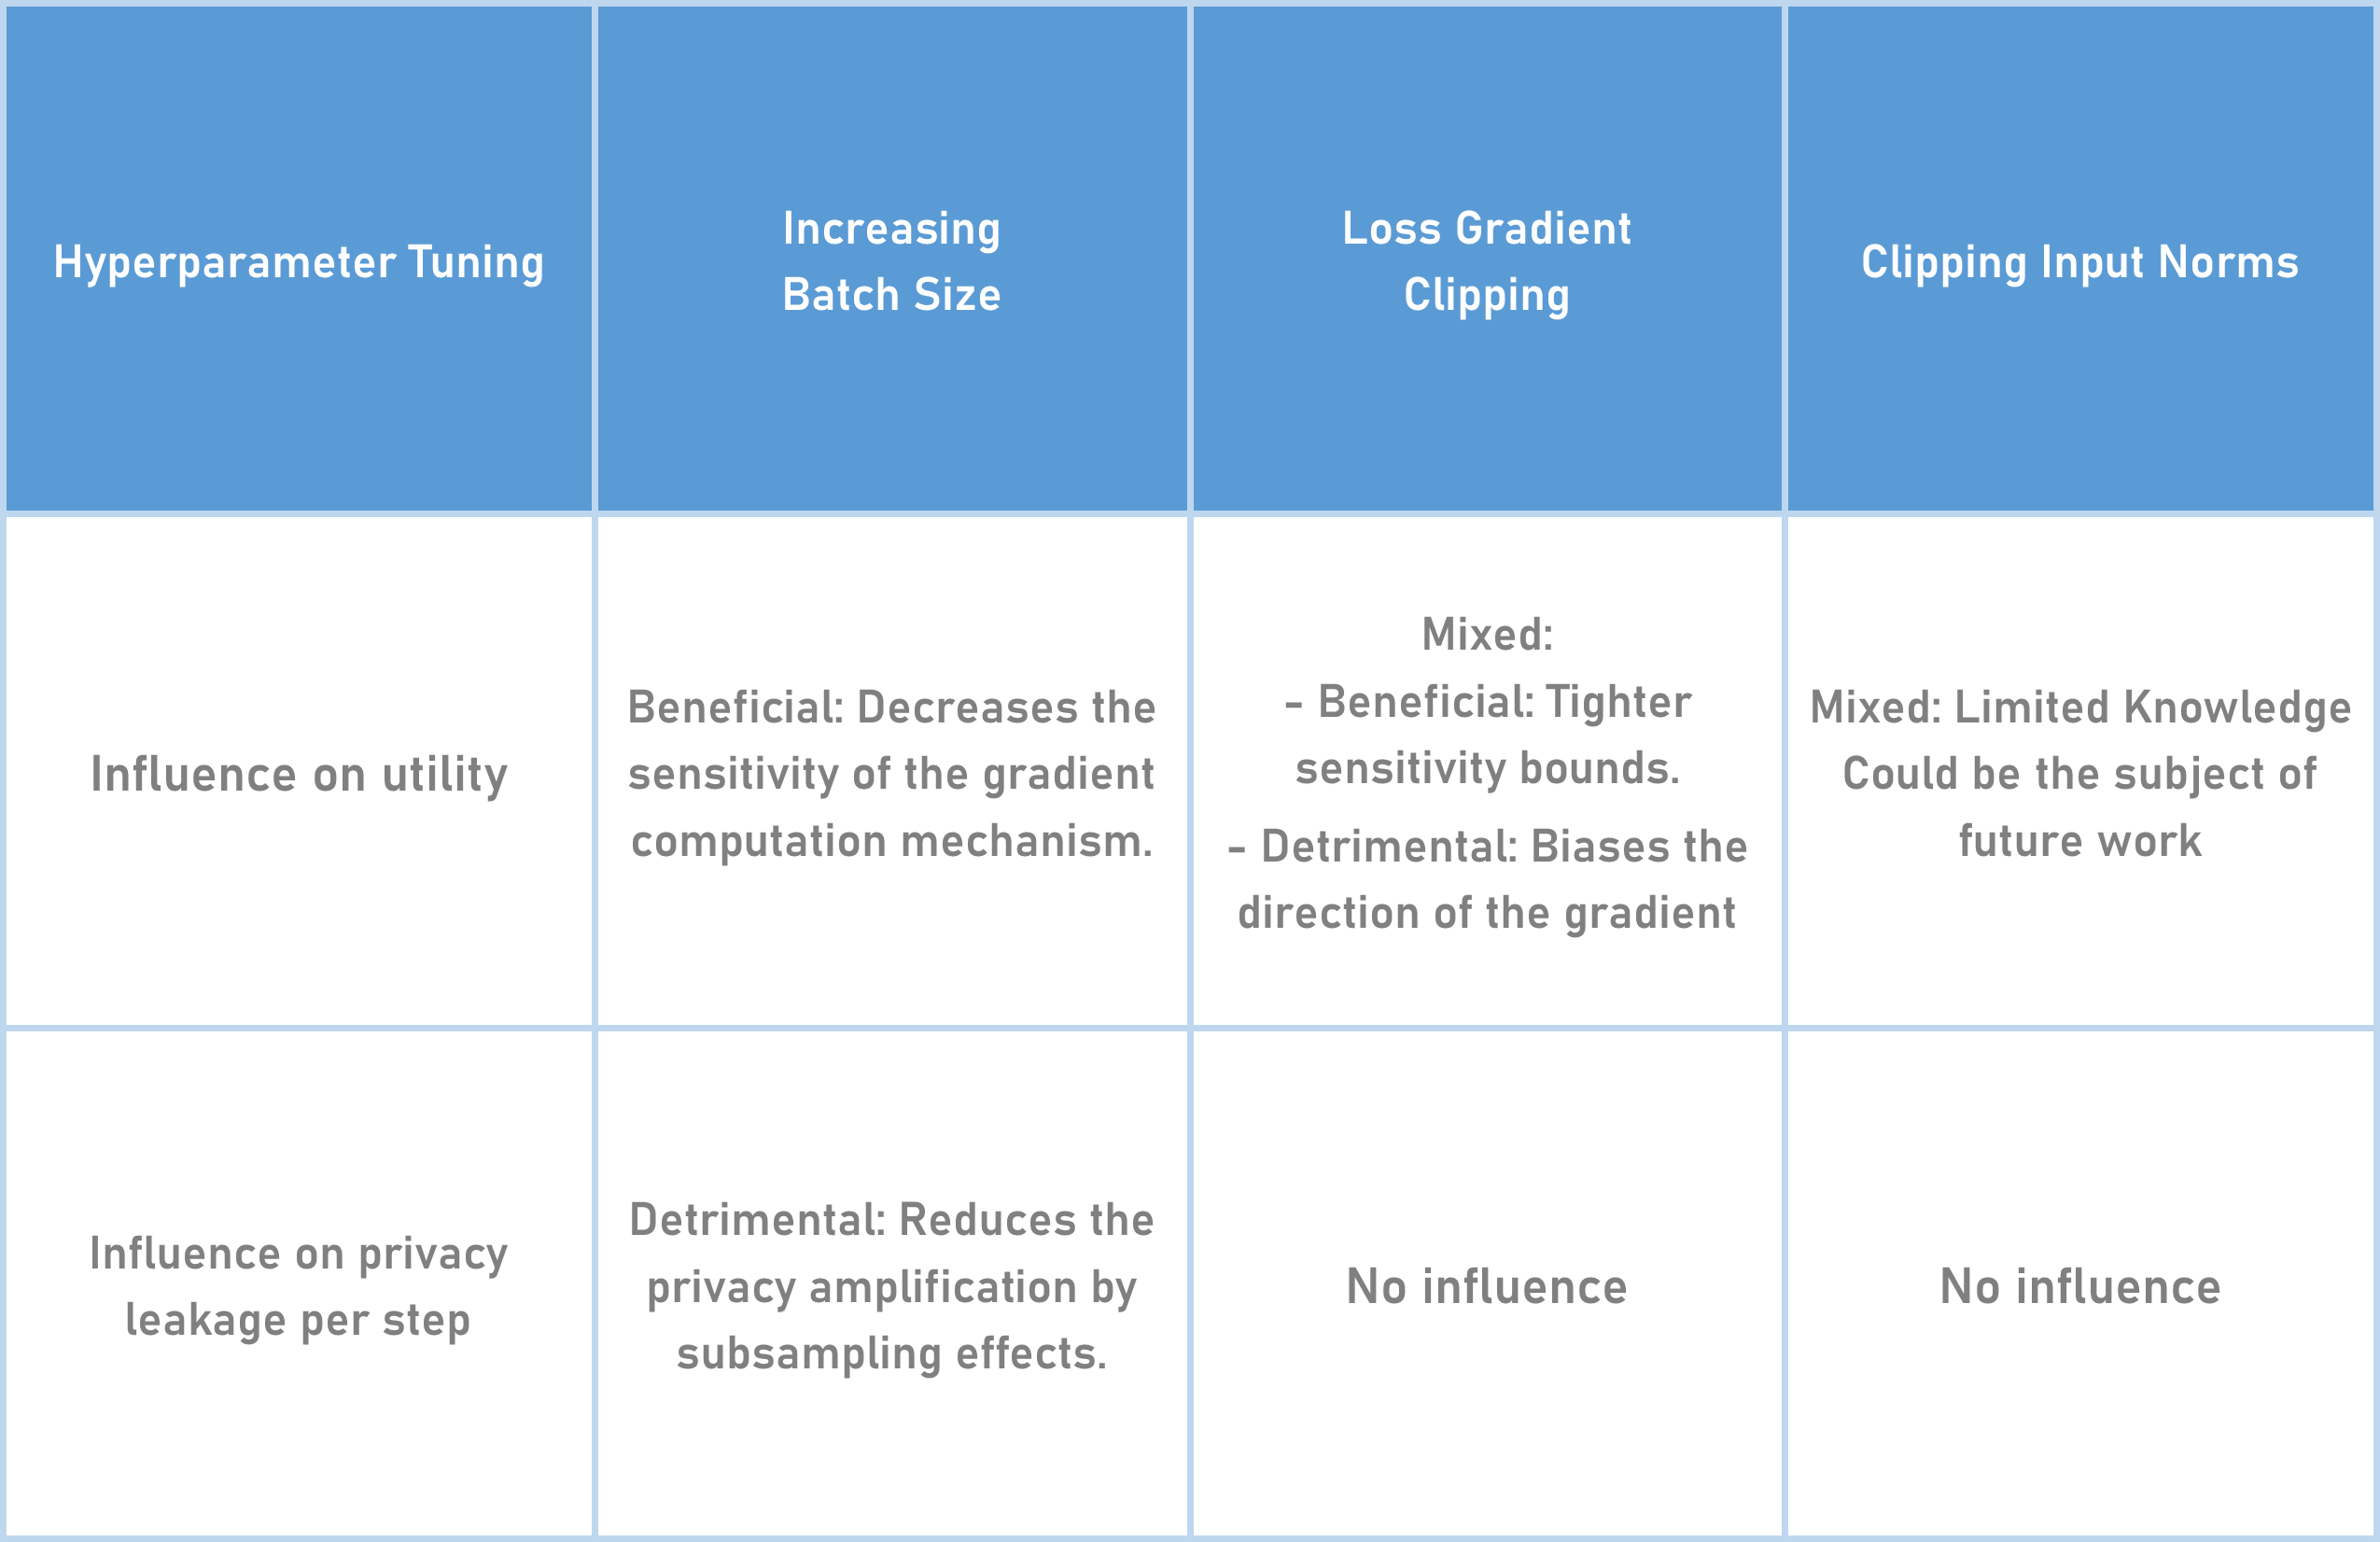
\includegraphics[width=0.7\linewidth,height=5.5cm]{figures/hyperparams.png}
    \caption{\textbf{Hyperparameter table:} Here, we give insights on the influence of some hyper-parameters on utility and privacy.}
    \label{fig:hyperparams}
\end{figure}

\subsubsection{Hyperparameters configuration for MNIST}

 Experiments are run on NVIDIA GeForce RTX 3080 GPUs. The losses we optimize are either the Multiclass Hinge Kantorovich Rubinstein loss or the $\tau-\text{CCE}$. 

\begin{center}
\begin{tabular}{|c c c|} 
 \hline
 Hyper-Parameter & Minimum Value & Maximum Value \\ [0.5ex] 
 \hline\hline
 Input Clipping & $10^{-1}$ & 1 \\ 
 \hline
 Batch Size & 512 & $10^4$ \\
 \hline
 Loss Gradient Clipping & \multicolumn{2}{c|}{automatic (90\%-th percentile)} \\
 \hline
 $\alpha$ (HKR) & $10^{-2}$ & $2,0 \times 10^3$ \\
 \hline
 $\tau$ (CCE) & $10^{-2}$ & $1,8 \times 10^{1}$ \\
 \hline
\end{tabular}
\end{center}

The sweeps were run with MLP or ConvNet architectures yielding the results presented in Figure~\ref{fig:paretofrontmnist}. 

\subsubsection{Hyperparameters configuration for FASHION-MNIST}

 Experiments are run on NVIDIA GeForce RTX 3080 GPUs. The losses we optimize are the Multiclass Hinge Kantorovich Rubinstein loss, the $\tau-\text{CCE}$ or the K-CosineSimilarity custom loss function. 
 
\begin{center}
\begin{tabular}{|c c c|} 
 \hline
 Hyper-Parameter & Minimum Value & Maximum Value \\ [0.5ex] 
 \hline\hline
 Input Clipping & $10^{-1}$ & 1 \\ 
 \hline
 Batch Size & $5.0 \times 10^3$ & $10^4$ \\
 \hline
 Loss Gradient Clipping & \multicolumn{2}{c|}{automatic (90\%-th percentile)} \\
 \hline
 $\alpha$ (HKR) & $10^{-2}$ & $2.0 \times 10^3$ \\
 \hline
 $\tau$ (CCE) & $10^{-2}$ & $4.0 \times 10^{1}$ \\
 \hline
 $K$ (K-CS) & $10^{-2}$ & $1.0$ \\
 \hline
\end{tabular}
\end{center}

A simple ConvNet architecture, in the spirit of VGG (but with Lipschitz constraints), was chosen to run all sweeps yielding the results we present in Figure~\ref{fig:paretofrontfashion}.

\subsubsection{Hyperparameters configuration for CIFAR-10}

 Experiments are run on NVIDIA GeForce RTX 3080 or 3090 GPUs. The losses we optimize are the Multiclass Hinge Kantorovich Rubinstein loss, the $\tau-\text{CCE}$ or the K-CosineSimilarity custom loss function. They yield the results of Figure~\ref{fig:paretofrontcifar}.

\begin{center}
\begin{tabular}{|c c c|} 
 \hline
 Hyper-Parameter & Minimum Value & Maximum Value \\ [0.5ex] 
 \hline\hline
 Input Clipping & $10^{-2}$ & 1 \\ 
 \hline
 Batch Size & $512$ & $10^4$ \\
 \hline
 Loss Gradient Clipping & \multicolumn{2}{c|}{automatic (90\%-th percentile)} \\
 \hline
 $\alpha$ (HKR) & $10^{-2}$ & $2.0 \times 10^3$ \\
 \hline
 $\tau$ (CCE) & $10^{-3}$ & $3.2 \times 10^{1}$ \\
 \hline
 $K$ (K-CS) & $10^{-2}$ & $1.0$ \\
 \hline
\end{tabular}
\end{center}

\begin{figure}%{r}{0.5\textwidth}
    %\vspace{-5mm}
    \center
    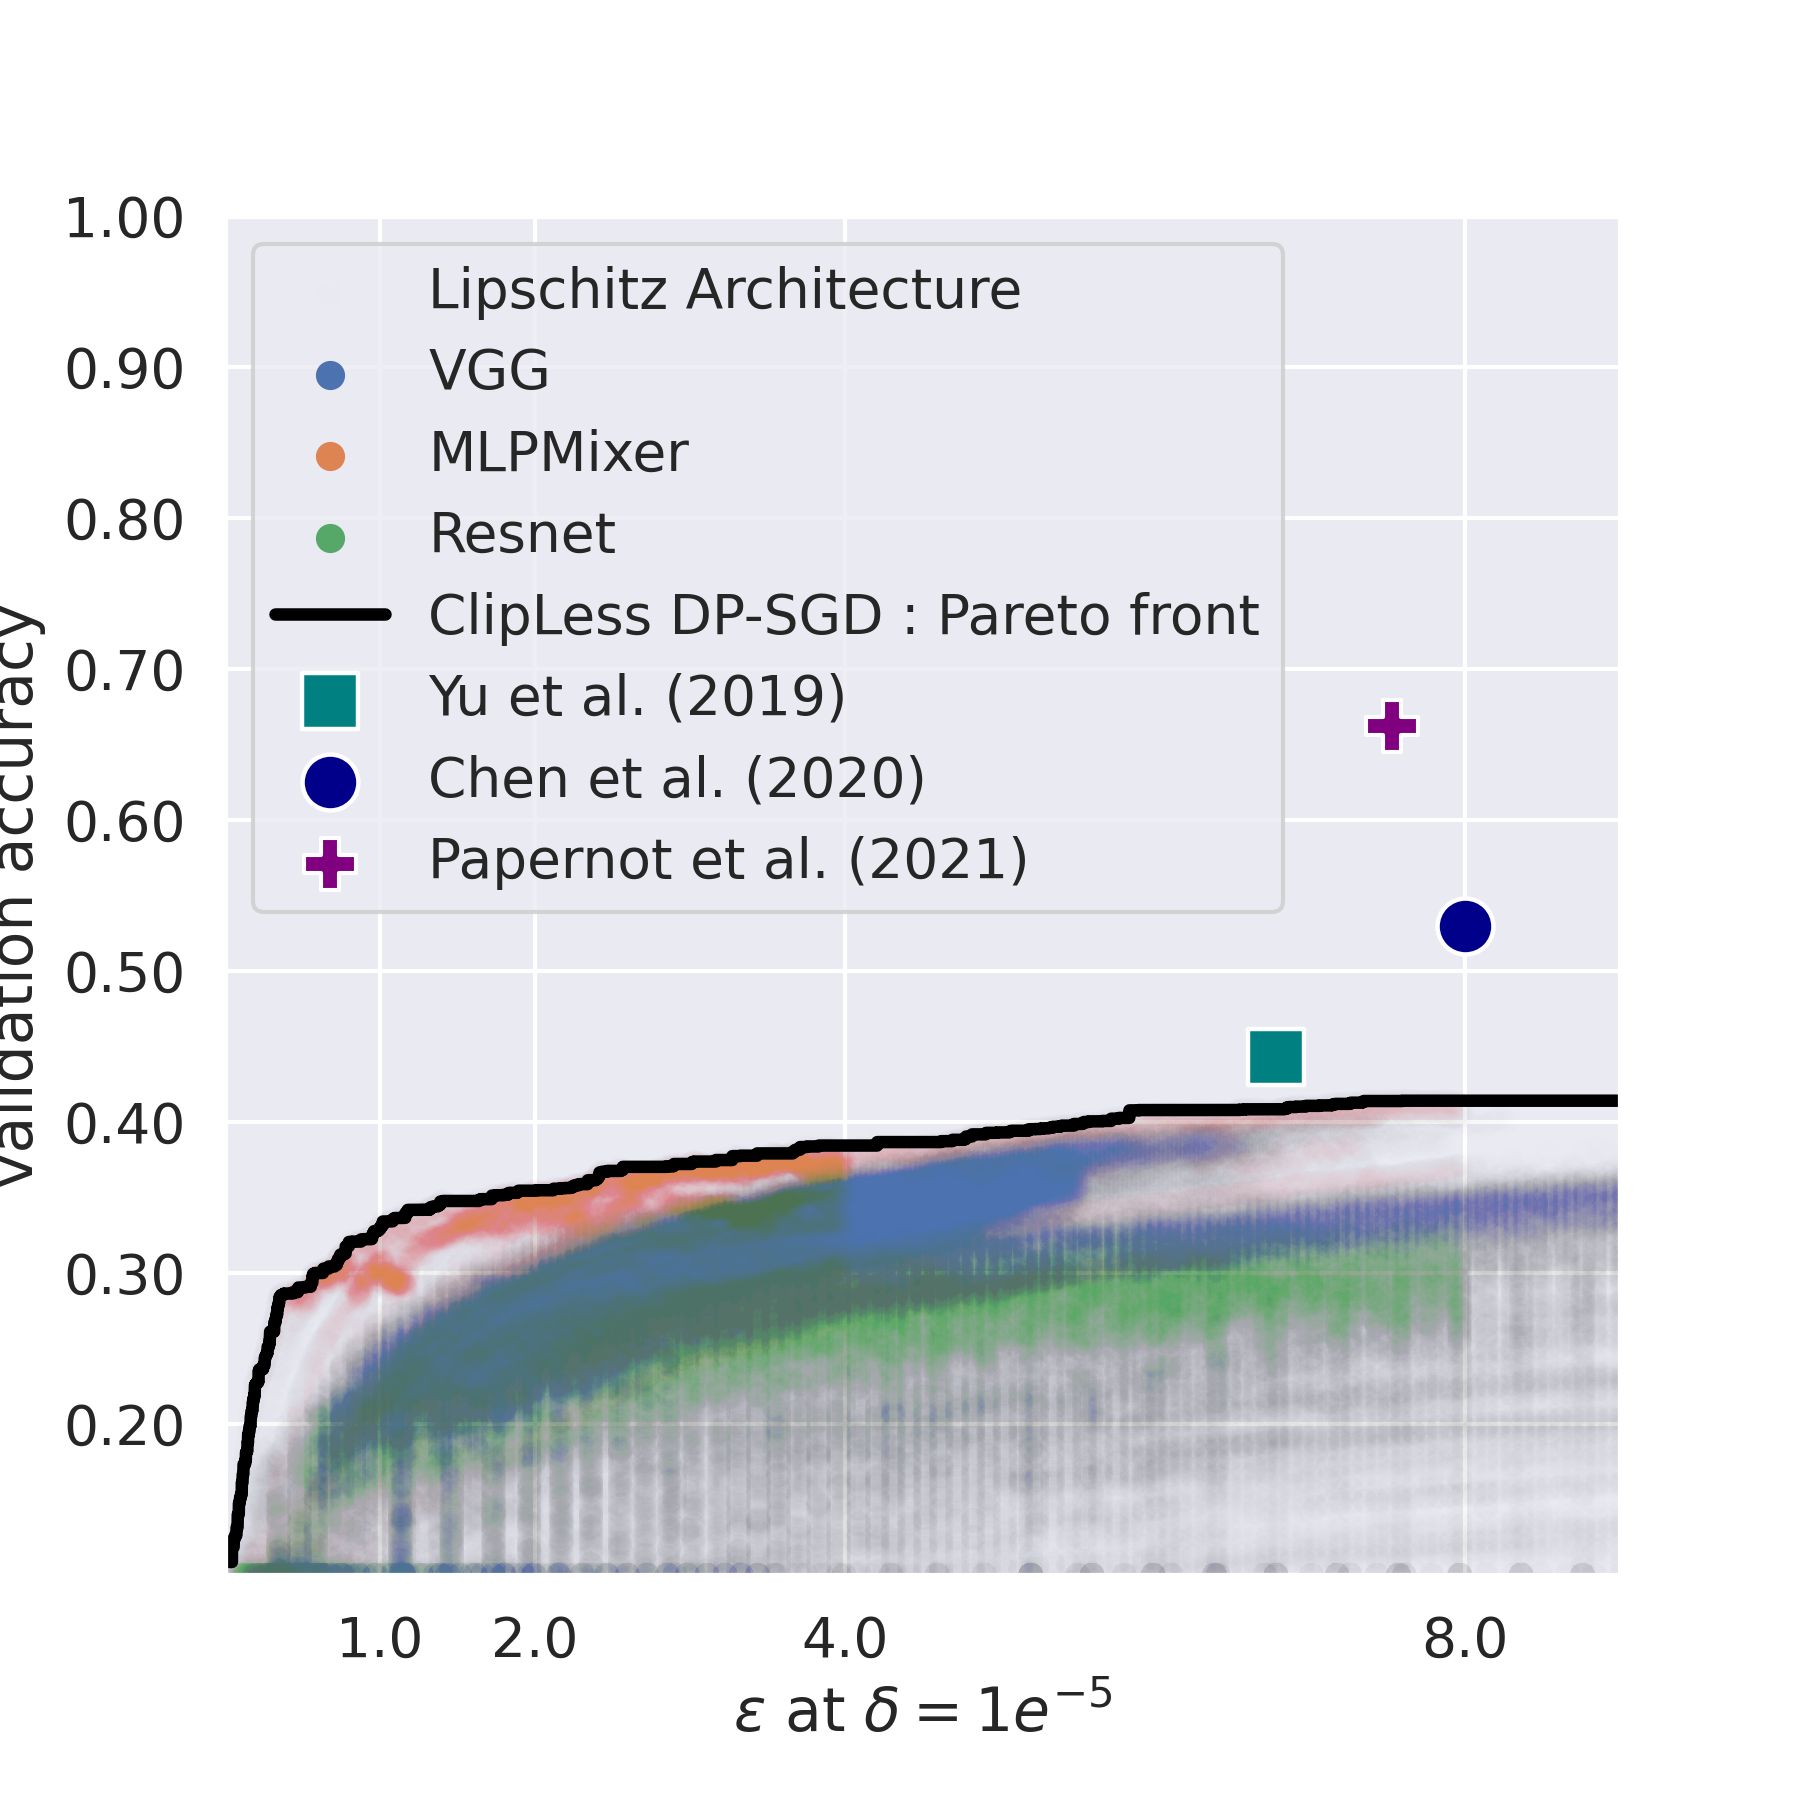
\includegraphics[width=0.45\textwidth]{figures/cifar10_per_architecture.png}
    \caption{Accuracy/Privacy tradeoff on Cifar-10, split down per architecture used. While some architectures seems to perform better than others, we don't advocate for the use of one over another. The results may not translate to all datasets, and may be highly dependant on the range chosen for hyper-parameters. While this figure provides valuable insights, identifying the best architecture is left for future works.}
    \label{fig:cifar10_allarch}
    %\vspace{-5mm}
\end{figure}

The sweeps have been done on various architectures such as Lipschitz VGGs, Lipschitz ResNets and Lipschitz MLP\_Mixer. We can also break down the results per architecture, in figure~\ref{fig:cifar10_allarch}. The MLP\_Mixer architecture seems to yield the best results.  This architecture is exactly GNP since the orthogonal linear transformations are applied on disjoint patches. To the contrary, VGG and Resnets are based on RKO convolutions which are not exactly GNP. Hence those preliminary results are compatible with our hypothesis that GNP layers should improve performance. Note that these results are expected to change as the architectures are further improved. It is also dependant of the range chosen for hyper-parameters. We do not advocate for the use of an architecture over another, and we believe many other innovations found in literature should be included before settling the question definitively.  

For the vanilla implementation of DP-SGD we rely on Opacus library. We use the default configuration from the official tutorial on Cifar-10, and we define the hyper-parameters for the grid search below:

\begin{center}
\begin{tabular}{|c c c|} 
 \hline
 Hyper-Parameter & Minimum Value & Maximum Value \\ [0.5ex] 
 \hline\hline
 Input & \multicolumn{2}{c|}{RGB standardized} \\ 
 \hline
 Batch Size & $500$ & $5000$ \\
 \hline
 Noise Multiplier & \multicolumn{2}{c|}{Automatic} \\
 \hline
 Epochs & 1 & 400\\
 \hline
 \makecell{Maximum\\ Gradient norm} & 0.01 & 100\\
 \hline
 \makecell{Learning rate} & $0.00001$ & 1\\
 \hline
\end{tabular}
\end{center}

\subsection{Configuration of the ``speed'' experiment}\label{sec:speedexperiment}

We detail below the environment version of each experiment, together with Cuda and Cudnn versions. We rely on a machine with 32GB RAM and a NVIDIA Quadro GTX 8000 graphic card with 48GB memory.
The GPU uses driver version 495.29.05, cuda 11.5 (October 2021) and cudnn 8.2 (June 7, 2021). We use Python 3.8 environment.

\begin{itemize}
    \item For Jax, we used jax 0.3.17 (Aug 31, 2022) with jaxlib 0.3.15 (July 23, 2022), flax 0.6.0 (Aug 17, 2022) and optax 1.4.0 (Nov 21, 2022).
    \item For Tensorflow, we used tensorflow 2.12 (March 22, 2023) with tensorflow\_privacy 0.7.3 (September 1, 2021).
    \item For Pytorch, we used Opacus 1.4.0 (March 24, 2023) with Pytorch (March 15, 2023).
    \item For lip-dp we used deel-lip 1.4.0 (January 10, 2023) on Tensorflow 2.8 (May 23, 2022).
\end{itemize}

For this benchmark, we used among the most recent packages on pypi. However the latest version of tensorflow privacy could not be forced with pip due to broken dependencies. This issue arise in clean environments such as the one available in google colaboratory.
% For our benchmarking, we only considered packages that can be installed out of the box from pip package manager.

% \subsection{Feature Visualizations of Lispchitz networks under DP training}
%     We apply the feature visualization of~\cite{olah2017feature} to monitor the features learned by (a) a conventional network (no DP training) (b) a GNP network (c) a GNP network with DP training.

\subsection{Compatibility with literature improvements}

Many method from the state of the art are based on improvement over the DP-SGD baseline. In this section we will review these improvements and check the compatibility with our approach.

\paragraph{Adaptive clipping.} As discussed in \ref{sec:gnp}, or approach can benefit from adaptive clipping. Similarly this can be done in a more efficient way.

\paragraph{Multiple augmentations} We tested adding ``multiple augmentation'' introduced by~\cite{de2022unlocking} on our approach but it did not yield improvements (see Appendix~\ref{fig:multipleaug}). This is probably due to the fact that we train our architecture from scratch: doing so require an architecture that requires a minimum amount of steps to converge. Such architecture are too small and not able to learn an augmented dataset as those are more prone to under-fitting.  Another reason is that in vanilla DP-SGD the elementwise gradients of each augmentation can be averaged \textit{before} the clipping operation, which has no consequences on the overall sensitivity of the gradient step. Whereas in our case, the average is computed \textit{after} the loss gradient clipping.

\begin{figure}
    \centering
    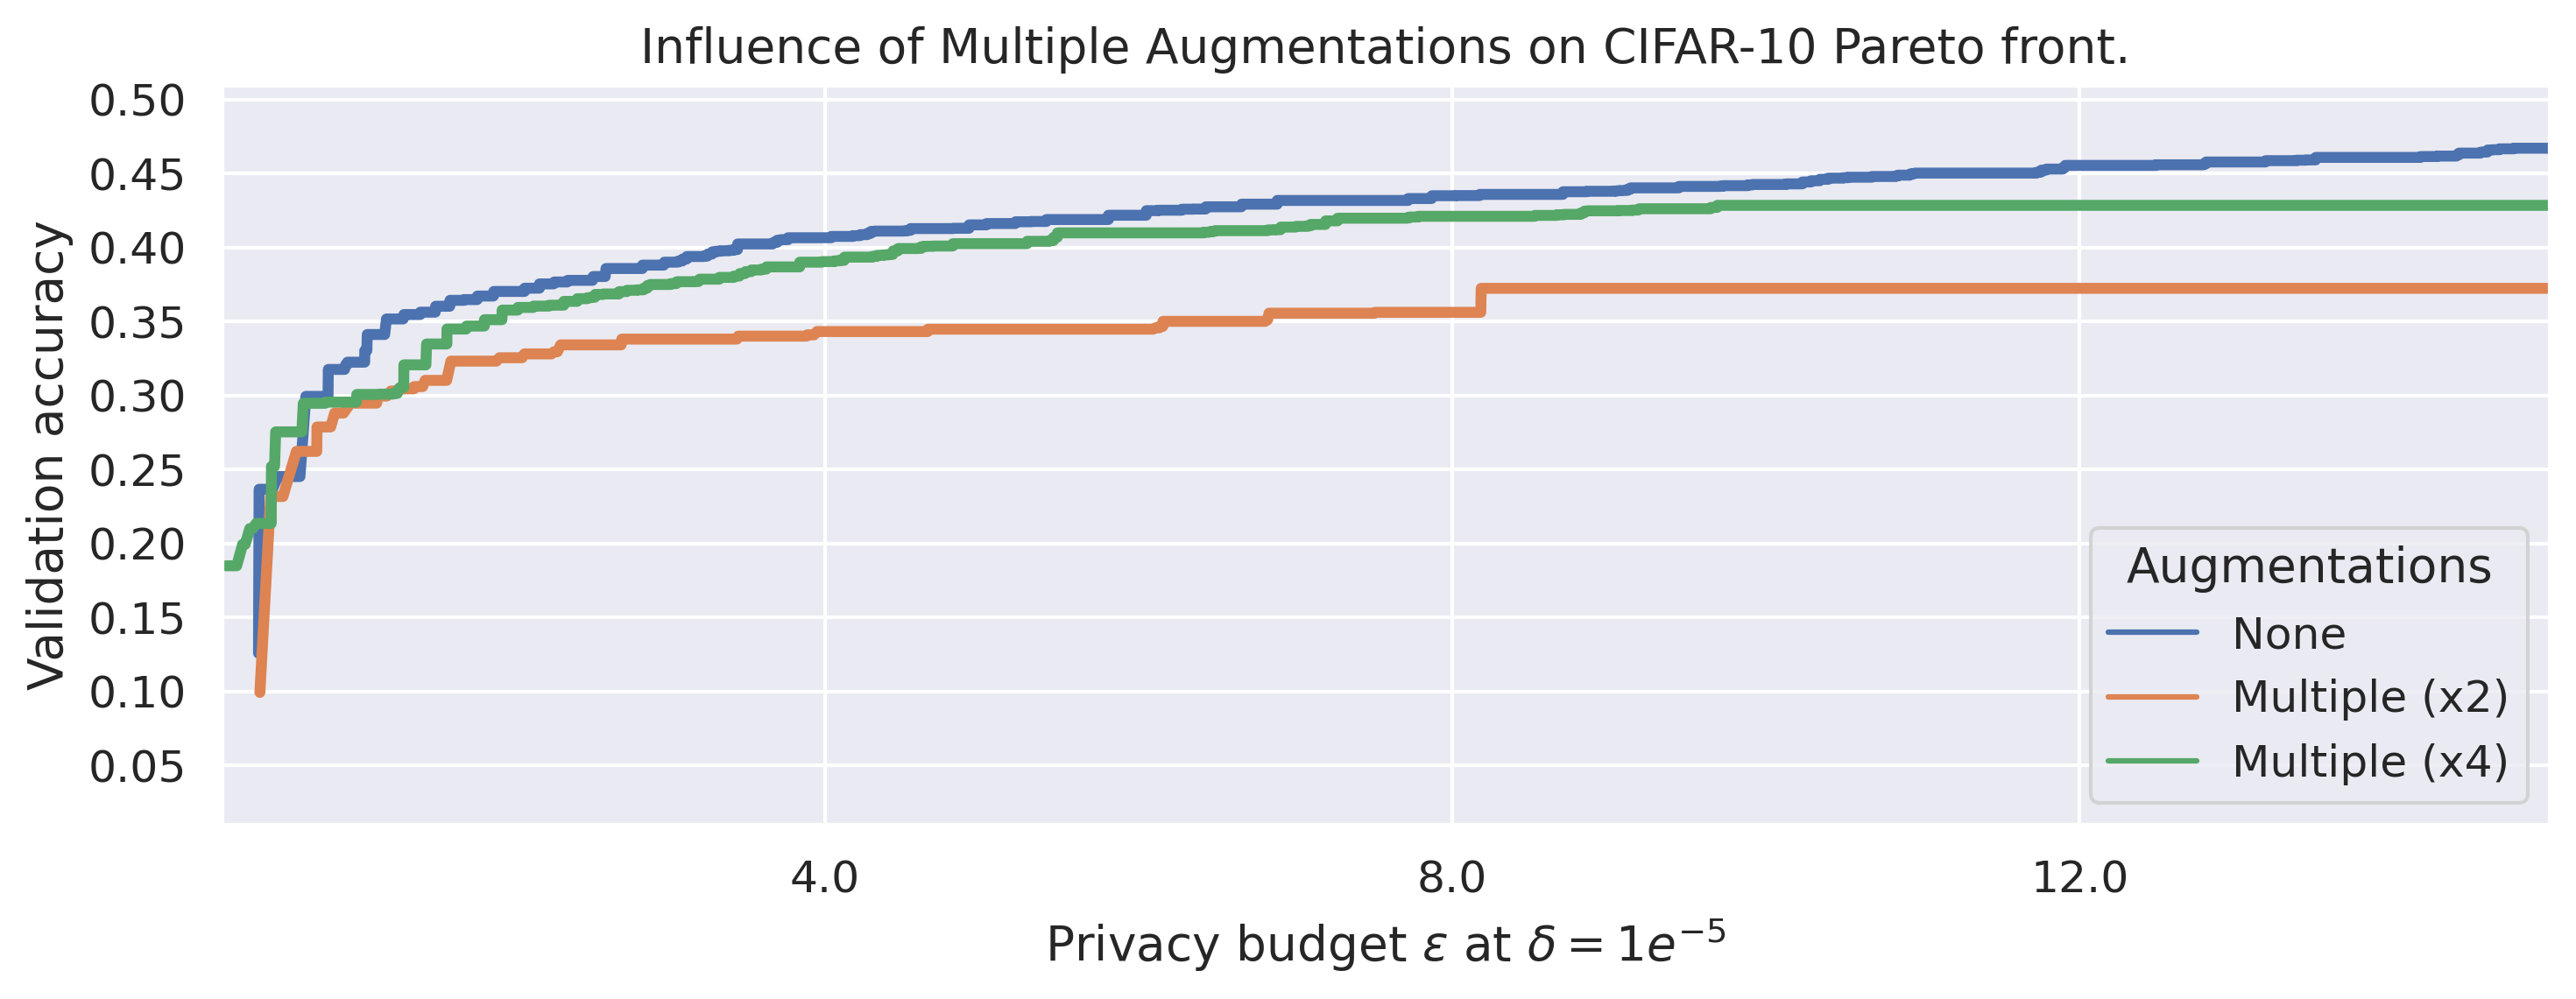
\includegraphics[width=\textwidth]{figures/multiaug.png}
    \caption{\textbf{Pareto front on Cifar-10 with the multiple augmentations trick of~\cite{de2022unlocking}}.}
    \label{fig:multipleaug}
\end{figure}

\paragraph{Fine tuning a pretrained backbone:} Clipless DP-SGD can work with a pre-trained backbone, however, the fine-tuned layers must be 1-lipschitz. This can yield 2 approaches:
\begin{itemize}
    \item \textbf{Using a 1-lipschitz backbone:} We can then fine tune the whole network and benefits from pre-training. Unfortunately there is no 1-lipschitz backbone available for the moment.
    \item \textbf{Using an unconstrained backbone:} Our approach can work with an unconstrained feature extractor using the following protocol: 1. the $n$ last layers are dropped and replaced with a 1-Lipschitz classification network. 2. An input clipping layer is added at the beginning of the classification head to ensure that the inputs are bounded. This approach was tested using a MobilenetV2 backbone. Results are reported in Figure~\ref{fig:finetuning}.
\end{itemize}

\begin{figure}
    \centering
    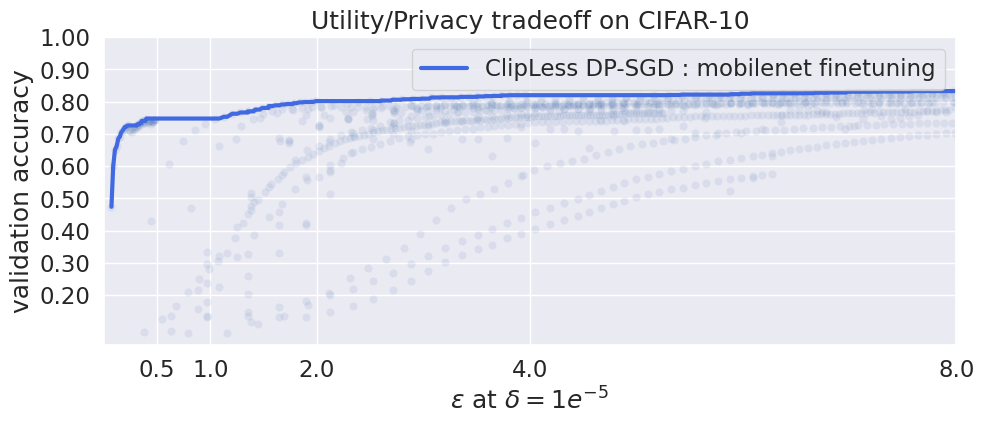
\includegraphics[width=\textwidth]{figures/mobilenet_finetuning.png}
    \caption{\textbf{Finetuning of a MobilenetV2 with Clipless DP-SGD.} A Lipschitz MLP (1 or 2 layers, and GroupSort activation) is trained using the backbone as a feature extractor. The backbone is not fine-tuned as it is not Lipschitz. Therefore a plateau exists, depending on the quality of the feature extractor.}
    \label{fig:finetuning}
\end{figure}

\subsection{Drop-in replacement with Lipschitz networks in vanilla DPSGD}\label{app:dropinreplacement}

     To highlight the importance of the tight sensitivity bounds $\Delta_d$ obtained by our framework, we perform an ablation study by optimizing GNP networks using ``vanilla'' DP-SGD (with clipping), in Figure~\ref{fig:vanillagnpmnist} and~\ref{fig:vanillagnpcifar}.

    Thanks to the gradient clipping of DP-SGD (see Algorithm~\ref{alg:dpsgd}), Lipschitz networks can be readily integrated in traditional DP-SGD algorithm with gradient clipping. The PGD algorithm is not mandatory: the back-propagation can be performed within the computation graph through iterations of Bj\"orck algorithm (used in RKO convolutions). This does not benefit from any particular speed-up over conventional networks - quite to the contrary there is an additional cost incurred by enforcing Lipschitz constraints in the graph. Some layers of deel-lip library have been recoded in Jax/Flax, and the experiment was run in Jax, since Tensorflow was too slow. 

    We use use the Total Amount of Noise (TAN) heuristic introduced in~\cite{sander2022tan} to heuristically tune hyper-parameters jointly. This ensures fair covering of the Pareto front.
    
    \begin{algorithm}%[tb]
    \caption{Differentially Private Stochastic Gradient Descent : \textbf{DP-SGD}}
    \label{alg:dpsgd}
    \textbf{Input}: Neural network architecture $f(\cdot,\cdot)$\\
    \textbf{Input}: Initial weights $\theta_0$, learning rate scheduling $\eta_t$, number of steps $N$, noise multiplier $\sigma$, L2 clipping value $C$ .\\
    \begin{algorithmic}[1] %[1] enables line numbers.
    \Repeat
        \For{\textbf{all} $1\leq t\leq N-1$}
        \State Sample a batch 
        $$\mathcal{B}_t = {(x_1, y_1), (x_2, y_2), \ldots , (x_b, y_b)}.$$
        \State Create microbatches, compute and clip the per-sample gradient of cost function:
            $$\tilde g_{t,i}\defeq \min(C,\|\nabla_{\theta_t} \Loss (\yhat_i,y_i)\|) \frac{\nabla_{\theta_t}\Loss (\yhat_i,y_i)}{\|\nabla_{\theta_t} \Loss (\yhat_i,y_i)\|}.$$
        \State Perturb each microbatch with carefully chosen noise distribution $b \sim \mathcal{N}(0,\sigma C)$ :
            $$\hat g_{t,i}\gets \tilde g_{t,i} + b_i.$$
        \State Perform projected gradient step:
            $$\theta_{t+1}\gets \Pi(\theta_t-\eta_t \hat g_{t,i}).$$
        \EndFor
    \Until{privacy budget $(\epsilon,\delta)$ has been reached.}
    \end{algorithmic}
    \end{algorithm}

    \begin{figure}
    \begin{subfigure}{.48\columnwidth}
        \centering
        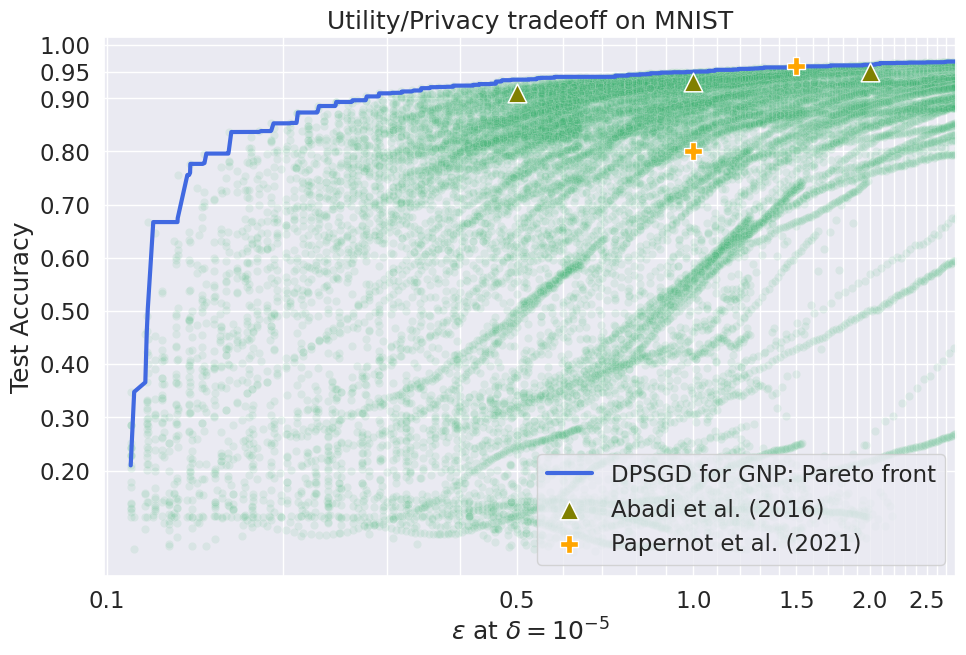
\includegraphics[width=\linewidth]{figures/mnistgnpvanilla.png}
        \caption{}
        \label{fig:vanillagnpmnist}
    \end{subfigure}
    \hfil
    \begin{subfigure}{.48\columnwidth}
        \centering
        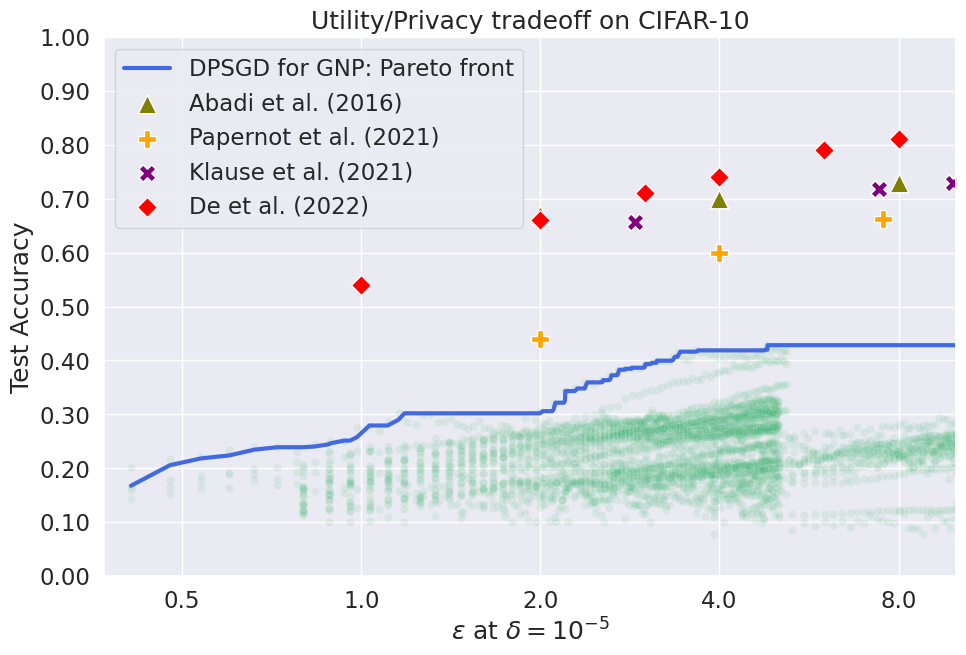
\includegraphics[width=\linewidth]{figures/cifargnpvanilla.png}
        \caption{}
        \label{fig:vanillagnpcifar}
    \end{subfigure}
    \caption{\textbf{Privacy/utility trade-off for Gradient Norm Preserving networks} trained under ``vanilla'' DP-SGD (\textbf{with} gradient clipping). Each green dot corresponds to a single epoch of one of the runs. Trajectories that end abruptly are due to the automatic early stopping of unpromising runs. Note that clipping + orthogonalization have a high runtime cost, which severely limits the number of epochs reported.}\label{fig:vaniallgnp}
    \end{figure}

\subsection{Extended limitations}

The main weakness of our approach is that it crucially rely on accurate computation of the sensitivity~$\sntv$. This task faces many challenges in the context of differential privacy: floating point arithmetic is not associative, and summation order can a have dramatic consequences regarding numerical stability~\cite{goldberg1991every}. This is further amplified on the GPUs, where some operations are intrinsically non deterministic~\cite{jooybar2013gpudet}. This well known issue is already present in vanilla DP-SGD algorithm. Our framework adds an additional point of failure: the upper bound of spectral Jacobian must be computed accurately. Hence Power Iteration must be run with sufficiently high number of iterations to ensure that the projection operator $\Pi$ works properly. The $(\epsilon,\delta)$-DP certificates only hold under the hypothesis that all computations are correct, as numerical errors can induce privacy leakages. Hence we check empirically the effective norm of the gradient in the training loop at the end of each epoch. No certificate violations were reported during ours experiments, which suggests that the numerical errors can be kept under control.  